% !TeX root = ../main.tex

\chapter{近邻图算法优化}
上一章中针对本文拟开展研究的基础进行了详细的阐述。本章立足于近邻图算法,首先在\ref{sec:galg-overview}节中指出现有\ganns 方法(以HNSW为代表)存在的问题和不足,分别是图连通性差和搜索过程存在冗余。然后在\ref{sec:galg-connection}节中针对图连通性差这一问题,进行分析并提出反向连接增强策略。在\ref{sec:galg-earlystop}节中针对搜索过程存在冗余这一问题,分析其原因并提出查询感知早停策略。


\section{概述}\label{sec:galg-overview}
尽管\ganns 方法相比其他类型的近似近邻搜索方法取得了成功,但其仍然存在诸多不足。首先,基于图的近似近邻搜索方法通常需要通过建立图来表示数据集。但是,当数据集的分布较为分散时,图的连通性可能会变得较差。这样的话,搜索算法就可能会错过一些真正接近查询点的近邻点。此外,在高维数据的情况下,基于图的近似近邻搜索方法也可能会遇到所谓的“维数灾难”问题,随着数据维数的增加,类似HNSW算法的多层图结构的效果变得越来越差,基本与单层图无异,因此本文中采用的都是单层图。其次,基于图的近似近邻搜索方法在搜索过程中还存在一些冗余。具体来说,由于它是基于图的方法,每个点都会与周围的一些点建立联系。然而,这些联系并不一定都是有意义的,有些联系甚至可能会干扰搜索算法的正常工作。

\subsection{图连通性差}
在\ganns 方法中,查询点根据图上点之间的连接,以迭代的方式查找它的相似点。因此,图索引的连通性对于最终的搜索结果至关重要。具体来说,某一点的入度越大,能找到它的点越多(搜索精度越高)。某个点的出度越大,每一步的搜索代价越大(搜索速度越慢)。一些入度较小的点的存在意味着图索引的连通性较差。对于某个查询点来说,如果这些入度较小的点属于查询点的真值,但在搜索过程中没有找到,则会导致较低的召回率。
本文通过实验来说明这一点,如图~\ref{fig:percent-in-degree}所示,以Turing1M数据集(详细的数据集介绍在\ref{sec:galg-experiment}节)为例。显然,某个点的入度越小,那么它对整体召回率的负面影响越大。对于入度较小(例如在这里小于19)的点,造成的召回率损失占总召回率损失的84.66\%。
% TODO:图片统一成htbp
\begin{figure}[htbp]
  \centering
  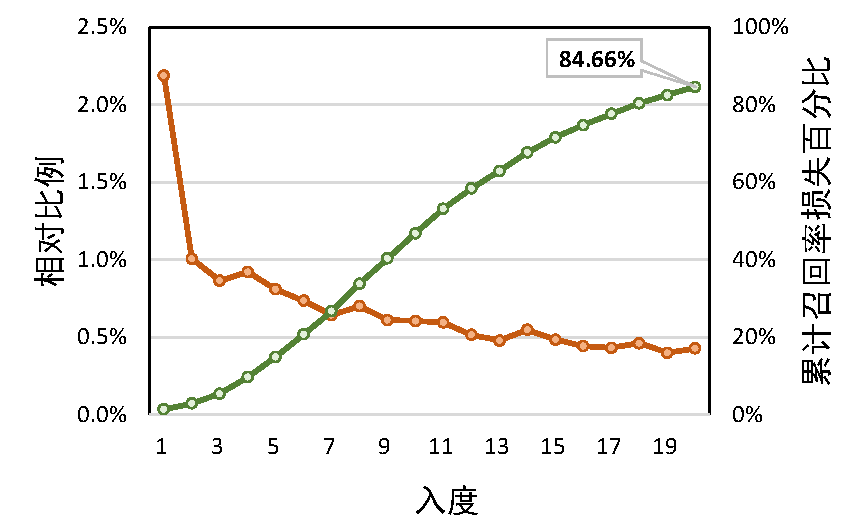
\includegraphics[width=0.7\textwidth]{figures/context-1/percent-in-degree.pdf}
  \caption{具有不同入度的点,对召回率损失的累积贡献曲线}
  \label{fig:percent-in-degree}
\end{figure}

本文指出,图连通性差的原因是由于现有构建算法的限制:即点的入度受其出度的限制。简单来说就是,为了保持图索引的高效性,一些点的出度会变小(通过近邻选择)。对于出度小的点,由于上述限制,它们的入度也小。接下来,本文将在\ref{sec:galg-connection}节中对这一限制的来源进行详细分析,并提出解决方案。


\subsection{搜索中存在冗余}
现有的最佳优先搜索算法在搜索过程中会产生较大的冗余,特别是在召回率较高的情况下。
正如本文在上一章节中所介绍的,$efs$参数是搜索算法中重要的超参数,它可以控制搜索速度和搜索精度(召回率)之间的权衡。总的来说,$efs$越大,精度越高,速度越慢。经过实验发现,$efs$参数与实际搜索过程中的迭代轮次(搜索步数)呈现出非常强的相关性。例如在$efs=200$的情况下,平均搜索步数为200.71,标准差为1.91。

因此为了简化问题的描述,本章节中的$efs$参数与搜索步数是相等的。为了便于叙述,本文首先定义\textit{最小搜索步数}:

\begin{definition}[最小搜索步数]
对于某个查询点$q_i$,在搜索步数$efs=s$下的召回率为$Recall_i$。那么存在一个保持$q_i$的召回率不降低的最小值$s$,那么$s$就是$q_i$在召回率为$Recall_i$的最小搜索步数。
\end{definition}
% 是搜索过程中结果队列的最大长度,每个查询的搜索步数数大致与$efs$成比例。

对于不同的查询点,其最小搜索步数差异很大。如图~\ref{fig:steps-histogram}所示,在DEEP1M数据集的查询集(有10000个查询点,详细见\ref{sec:galg-experiment}节)上,超过40\%查询点的最小搜索步数小于39。然而,现有的搜索算法对查询集中的所有查询点都设置相同的$efs$参数,在图~\ref{fig:steps-histogram}中这个值是300。
因此,现有搜索算法在搜索中就存在严重的冗余。对于上述那些最小搜索步数小于39的查询点,有87\%的搜索开销是冗余的(34.8\%的整体冗余开销)。接下来,我们将在\ref{sec:galg-earlystop}节中详细分析这个问题的原因,并提出我们的解决方案。

\begin{figure}[htbp]
  \centering
  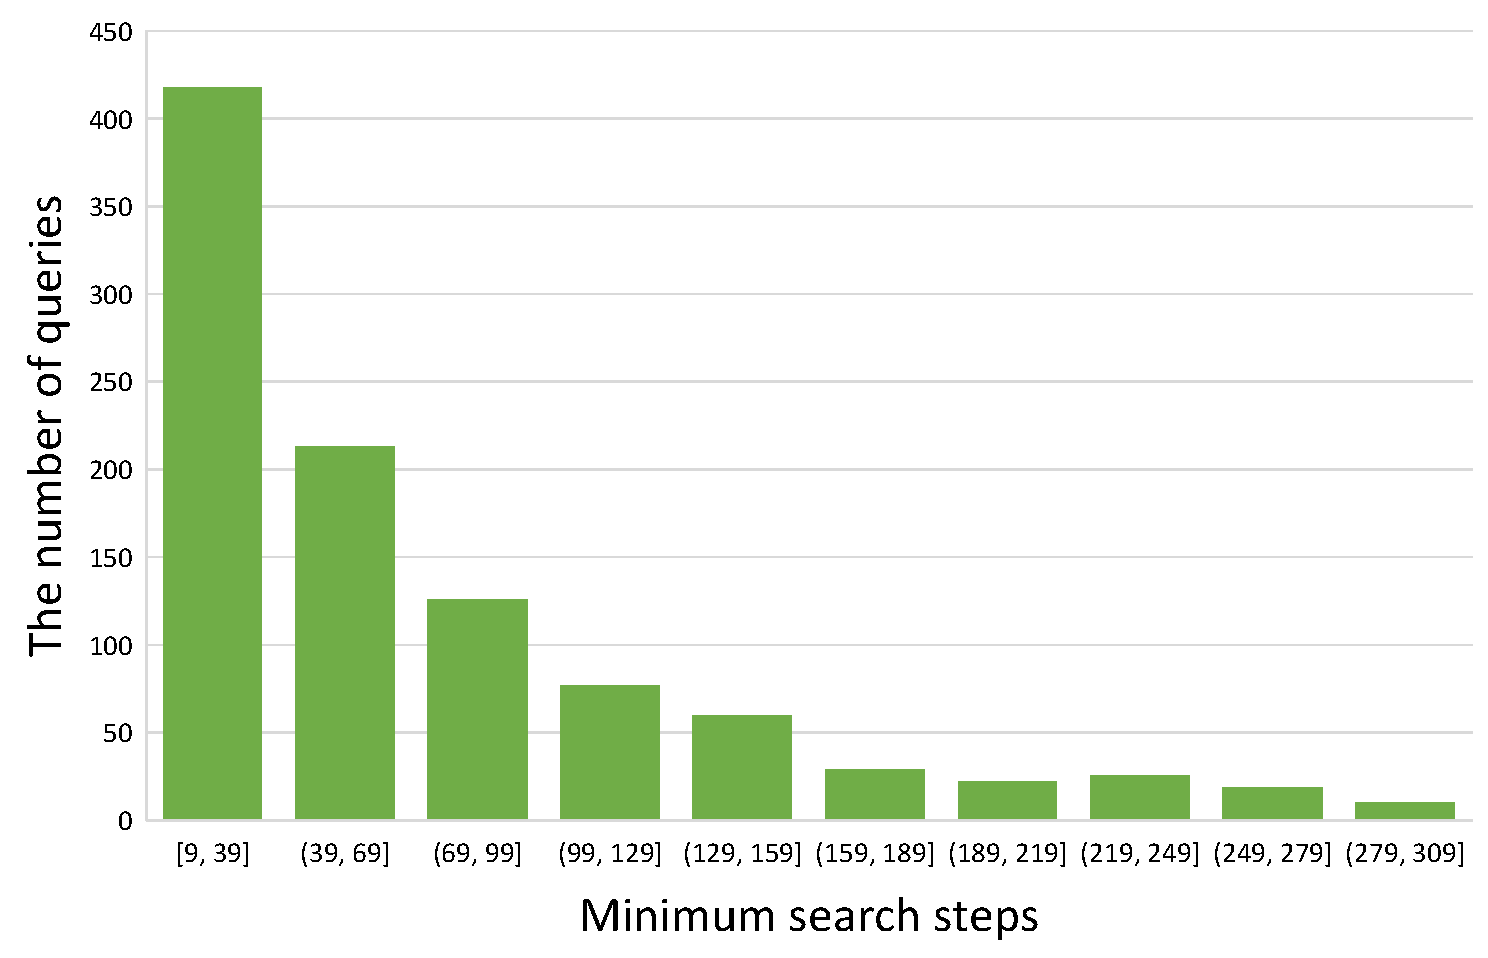
\includegraphics[width=0.7\textwidth]{figures/context-1/steps-histogram.pdf}
  \caption{查询集的最小搜索步数分布直方图\todo{重新画图}}
  \label{fig:steps-histogram}
\end{figure}

% todo:方法介绍?
\section{反向连接增强策略}\label{sec:galg-connection}
% TODO:表述到底是图还是图索引?
由于图中具有较小入度的点会对最终结果造成严重的精度影响,因此本节首先对整个HNSW图的入度和出度进行了分析,指出该问题的来源是现有构建算法不合理的限制。最后本文提出反向连接增强策略,有效减少这一问题导致的精度下降。

\subsection{度分析}
构建过程就是将数据集$X$中的数据点逐一添加到图上。如图~\ref{fig:idg-odg}所示,在时间$t_c$处,对应的待添加点是$x_c$(也称为插入点),此时对应的图是$G_c$。从点$x_c$的视角来看,整个构建过程可以分为两个部分:$t_c$之前和$t_c$之后。那么相应的,$x_c$的入度$IDG(x_c)$和出度$ODG(x_c)$也可以表示为两部分,如下公式所示:
\begin{equation}
  IDG(x_c) = IF1_{x_c} + IF2_{x_c}
\end{equation}
\begin{equation}
  ODG(x_c) = OF1_{x_c} + OF2_{x_c}
\end{equation}

\begin{itemize}
  \item $OF1_{x_c}$:在时间$t_c$之前$x_c$增加的出度。具体来说,当构建过程中插入点为$x_c$时(在图~\ref{fig:idg-odg}中$t_c$之前),在图索引$G_c$(在$t_c$之前)中找到$x_c$的$efc$最近点称为候选点。我们通过基于RNG的邻居选择策略选择其中的一部分作为$x_c$的邻居(即:$Neighbor(x_c)$),这些邻居的数量是$OF1_{x_c}$。
  \item $IF1_{x_c}$:在时间$t_c$之前$x_c$增加的入度。具体来说,在构建过程中插入点为$x_c$时(在图~\ref{fig:idg-odg}中为$t_c$之前),我们选择了$x_c$的当前邻居$Neighbor(x_c)$。对于$Neighbor(x_c)$中的每个点,当其邻居的数量小于$maxM0$时,我们还需要添加$x_c$作为其邻居。最终成功添加$x_c$作为邻居的点数是$IF1_{x_c}$,显然是$IF1_{x_c} \leq OF1_{x_c}$。
  \item $IF2_{x_c}$:在时间$t_c$之后$x_c$增加的入度。具体来说,当$x_c$已经在图中(在图~\ref{fig:idg-odg}中的$t_c$之后),$x_c$也可能成为其他插入点(绿色点)的候选点。如果点$x_c$最终成为了这些插入点的邻居,那么也就意味着$x_c$的入度会相应增加,增加的大小为$IF2_{x_c}$。
  \item $OF2_{x_c}$:在时间$t_c$之后$x_c$增加的出度。具体来说,当$x_c$已经在图索引中(在图~\ref{fig:idg-odg}中$t_c$之后),并且有一些点(黄色点)添加了$x_c$作为邻居。然后我们还需要将这些点添加为$x_c$的邻居,当$Neighbor(x_c)$的数量小于$maxM0$时。$x_c$的新邻居数量是$OF2_{x_c}$。
\end{itemize}

\begin{figure}[htbp]
  \centering
  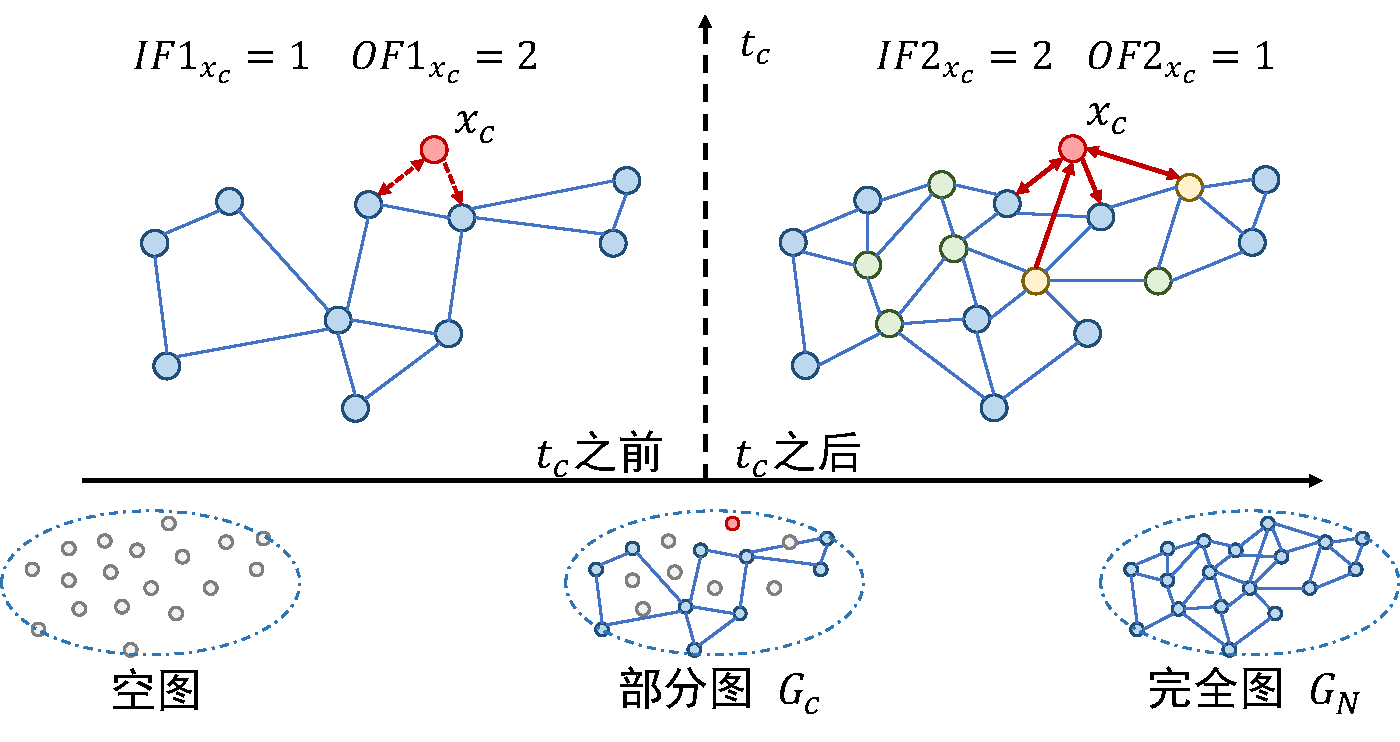
\includegraphics[width=0.7\textwidth]{figures/context-1/idg-odg.pdf}
  \caption{点$x_c$的入度和出度分别由两部分组成}
  \label{fig:idg-odg}
\end{figure}

\begin{figure}[tp]
  \centering
  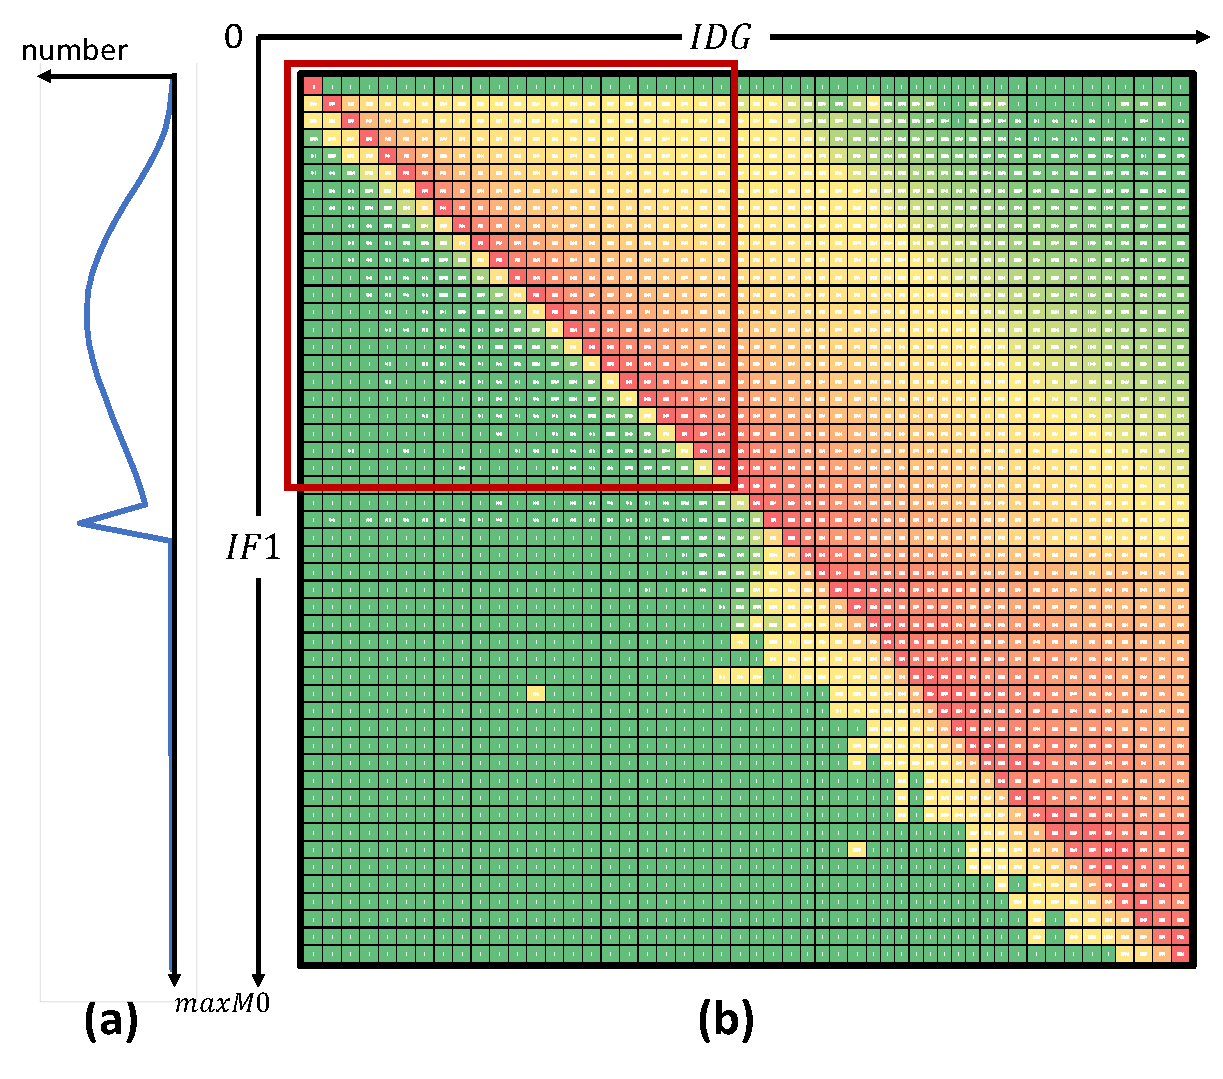
\includegraphics[width=0.6\textwidth]{figures/context-1/IF1-IDG.pdf}
  \caption{(a) $IF1$图索引上所有点的分布曲线(在Turing1M数据集上)。(b) $IDG$和$IF1$的热图,对于入度较小的点(在红框内),两者之间存在正相关关系。矩阵的每一行都按照(a)进行归一化。单个点的In-degree(约0.3 \textperthousand)非常大($\geq maxM0$),我们将它们截断。}
  \label{fig:if1-idg}
\end{figure}

如图~\ref{fig:idg-odg}所示, $IF2_{x_c}$和$OF2_{x_c}$取决于$x_c$是否可以被其他点(绿色点)找到。显然,入度$IF1_{x_c}$在$t_c$上的值越大,在$t_c$之后发现$x_c$的概率就越大。图~\ref{fig:if1-idg}(b)展示了$IDG$和$IF1$之间的关系。如果某些点(红框内)的$IF1$很小,那么它们最终入度$IDG$也很小。也就是说,$IDG$和$IF1$之间存在正相关关系。

在完整图$G_N$中的点$x_c$的连通性很大程度上取决于$IF1_{x_c}$。同时,$IF1_{x_c}$与$OF1_{x_c}$之间存在着一种\textbf{制约关系},即$IF1_{x_c} \leq OF1_{x_c}$。基于RNG的近邻选择策略尽管可以保持图上搜索\cite{hnsw-2018}的较高效率,但是忽略了对于这些入度较小点的关注。这导致了80.5\%的点$OF1$小于$maxM0$的2/5(如图~\ref{fig:if1-idg}(a),因为$IF1$和$OF1$的分布几乎相同)。也就是说,$IF1_{x_c}$与$OF1_{x_c}$之间存在制约关系,最终导致图$G_N$的连通性差。

\begin{algorithm}[tp]
  \caption{反向连接增强算法}
  \label{alg:enhancement} 
  \begin{algorithmic}[1]
      \REQUIRE
      底库数据集 $X$, 最大邻居数 $maxM0$, 起始点 $p_s$
      \ENSURE
      图索引 $G_N$
      \FOR{ $p_{in} \in X$}
      \STATE $Q_{cand}^{in} \gets$ greedy search$(q,G_s,p_s,efc,efc)$
      \STATE $Q_{sel}^{in} \gets$ SelectNeighborByRNG$(p_{in},Q_{cand}^{in},maxM0)$
      \STATE $setNeighbor(p_{in}) \gets Q_{sel}^{in}$
      \STATE $Q_{add} \gets Q_{cand}^{in} \setminus Q_{sel}^{in}$
      \FOR{ $p_r \in Neighbor(p_{in})$}
      \STATE $addNeighbor(pr) \gets p_{in}$
      \ENDFOR
      
      \WHILE{$Indegree(p_{in}) < maxM0$}
      \STATE $p_r \gets Q_{add}$
      \STATE $addNeighbor(pr) \gets p_{in}$
      \ENDWHILE
      \ENDFOR
      \RETURN $G_N$
  \end{algorithmic} 
\end{algorithm}

\subsection{我们的方法}
为了解决上述问题,本文提出了反向连接增强策略。我们对入度小的点增加了一些连接,使$IF1$打破了与$OF1$的限制关系。简单来说,点$x_c$的入边不仅从其邻居中选择,而且从其候选点中也考虑一部分,由于候选点是已经计算过的,因此也不会导致额外的计算开销。这一策略的伪代码如算法~\ref{alg:enhancement}所示。

图~\ref{fig:enhence}直观地展示了反向连接增强策略,$x_c$是构建过程中的插入点,($x_1$, $x_2$, $x_3$)是$x_c$的候选集。然后通过基于RNG的邻居选择策略选择$x_1$和$x_3$作为$x_c$的邻居。我们的方法和之前的方法的区别主要体现在$IF1_{x_c}$。因为$x_2$和$x_4$比$x_c$更接近$x_3$,所以$x_c$不属于$Neighbor(x_3)$。由于$OF1_{x_c}$受限于$IF1_{x_c}$,以前的方法只能通过$x_1$找到$x_c$,这意味着其他点很难找到$x_c$。
我们的方法打破了$IF1_{x_c}$和$OF1_{x_c}$之间的限制关系,从$x_c$的候选点中选择一些点(如$x_2$),然后将$x_c$作为$x_2$的邻居(用紫色的边连接)。然后我们可以通过$x_1$或$x_2$点找到$x_c$。与之前的方法相比,该方法极大地提高了图的连通性。详细的比较结果显示在\ref{sec:galg-experiment}部分。

\begin{figure}[htbp]
  \centering
  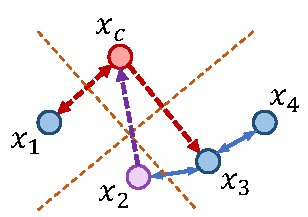
\includegraphics[width=0.4\textwidth]{figures/context-1/enhance.pdf}
  \caption{反向连接增强策略。之前:只能通过点$x_1$找到点$x_c$,现在:通过点$x_1$或点$x_2$都可以找到点$x_c$。}
  \label{fig:enhence}
\end{figure}


\section{查询感知早停策略}\label{sec:galg-earlystop}
现有的最佳优先搜索算法在搜索过程中会产生较大的冗余,特别是在召回率较高的情况下。其原因是不同的查询点所处的图区域不同,因此对于不同的查询都采用相同的搜索步数会造成严重的计算冗余问题。本节首先对这一问题进行分析,指出查询之间的最小搜索步数的差异来源是由于所处图区域的连接特点不同。然后提出查询感知早停策略,可有效减少搜索算法在召回率较高情况下的冗余。

\subsection{分析}
本文指出,查询在图上的区域连接关系导致了冗余搜索问题,区域是指图中靠近查询的部分。对于相同的查询,其最小搜索步数在不同的图上的差异很大。
图~\ref{fig:min-step}显示了查询向量的最小搜索步数的分布(在DEEP1M数据集上),水平轴和垂直轴分别对应两个不同的图索引。这两个图索引具有相同的基向量和参数,并且在构建过程中只改变插入点的顺序。我们发现对于相同的查询,其最小搜索步数之间有巨大的差异(例如,3到190)。
\begin{figure}[htbp]
  \centering
  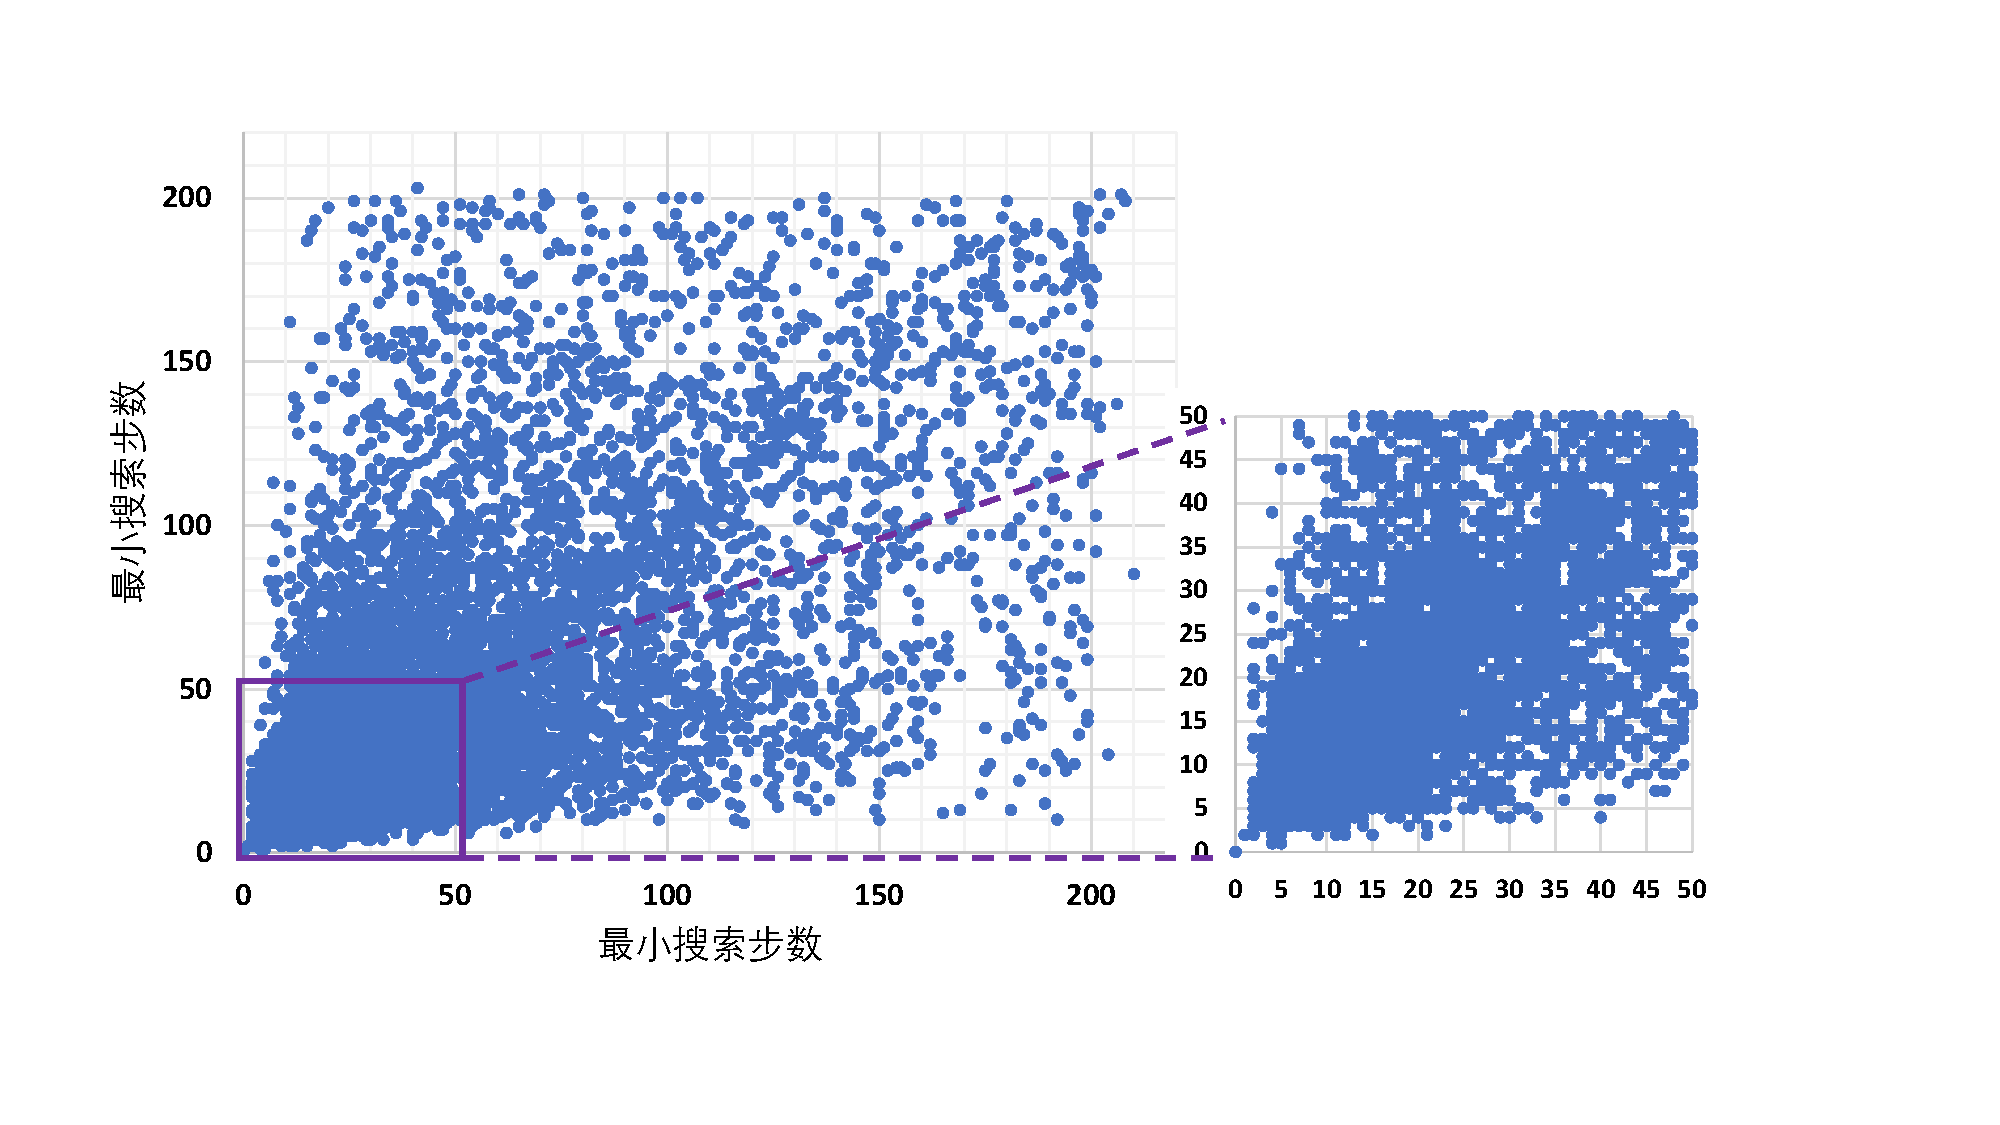
\includegraphics[width=0.9\textwidth]{figures/context-1/min search step.pdf}
  \caption{查询向量的最小搜索步数分布在两个不同的图索引中}
  \label{fig:min-step}
\end{figure}

根据连接关系的特点,区域可分为两种类型:对称连接区域(图~\ref{fig:grid}(a))和非对称连接区域(图~\ref{fig:grid}(b))。对称连接是指某一点的邻居在空间中均匀分布。非对称连接是指某一点的邻居在空间上不均匀分布。
与对称连接区域相比,非对称连接区域需要更多的搜索步数才能达到相同的召回率。 
当当前搜索点非常接近查询时。对于对称连接区域,当前搜索点可以快速地对查询的附近区域进行完整的探索。因此,对称连接区域可以以较少的搜索步数找到查询的所有最近点。对于非对称连接区域,由于查询附近的点之间缺乏连接,当前搜索点会采取一些“绕路”的方式来寻找所有与查询最近的点。 如图~\ref{fig:grid}所示,$q_a$的最小搜索步数仅为7步,$q_b$的最小搜索步数高达17步。如果我们想要得到同样高的召回率,那么在$q_a$的搜索开销中存在冗余。
\begin{figure}[tp]
  \centering
  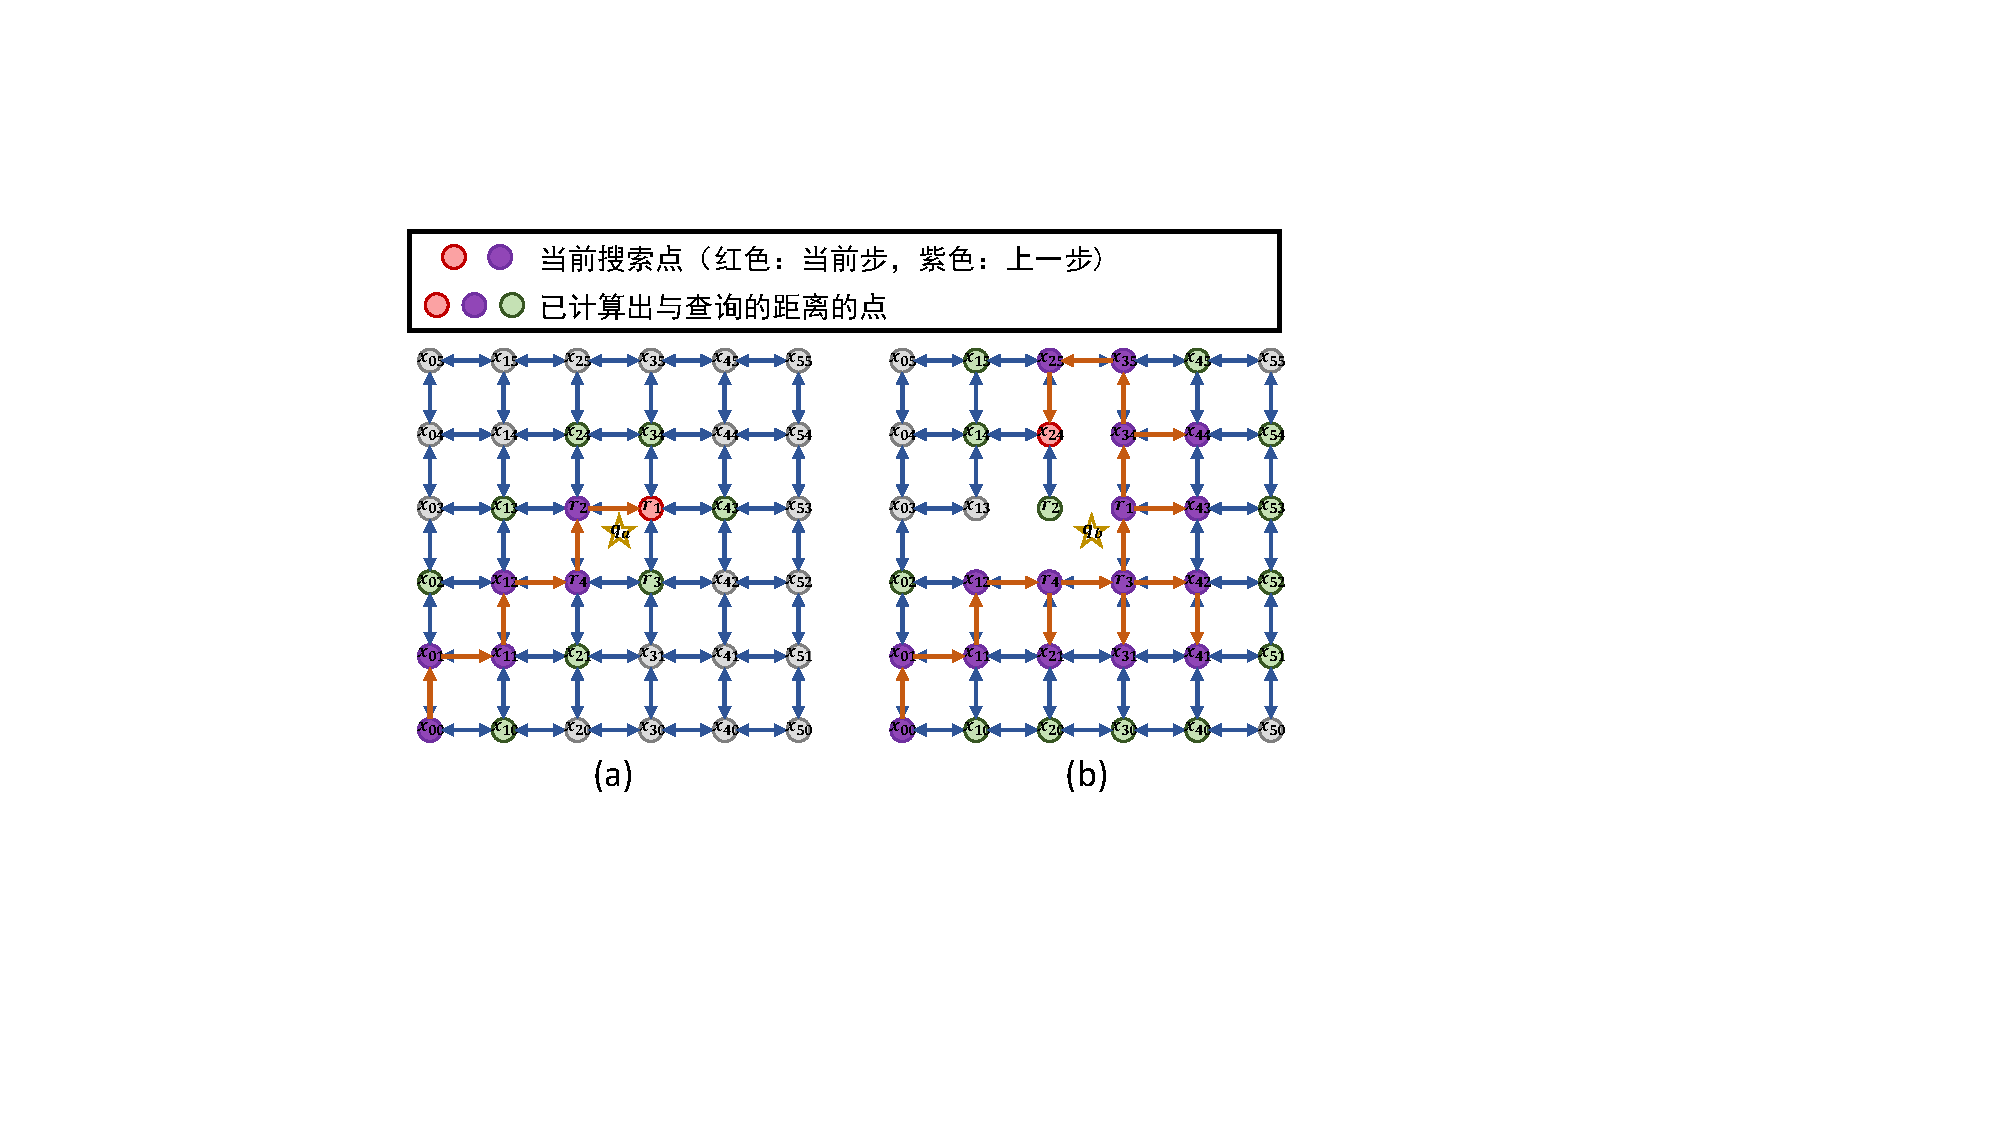
\includegraphics[width=0.6\textwidth]{figures/context-1/grid.pdf}
  \caption{在图索引上搜索查询最近邻的示意图。(a)当查询$q_a$位于一个对称连接区域时,可以很容易地找到它的所有最近邻居。(b)当查询$q_b$位于非对称连接区域时,我们需要更多的搜索步数来找到所有的最近邻居。}
  \label{fig:grid}
\end{figure}

由于高维空间中的连接关系非常复杂,从构建算法上很难解决该问题。因此,本文从搜索算法的角度来解决这个问题。
我们定义两个变量$d_{pop}$和$d_{topk}$来识别区域的连接关系。这里的距离是指某个点与查询之间的距离。对于搜索过程的每个步骤,$d_{pop}$表示当前搜索点的距离,$d_{topk}$表示从结果队列中$k$ -th最近的点到查询的距离。

我们通过在搜索过程中$d_{pop}$和$d_{topk}$的变化来识别这两种类型的区域。当当前搜索点非常接近查询时,如果曲线$d_{pop}$相对于曲线$d_{topk}$是光滑的,则意味着区域连接关系是对称的。
对于对称连接区域,由于邻居分布非常均匀,靠近查询的点将被添加到搜索队列中。因此,曲线$d_{pop}$相对于曲线$d_{topk}$是光滑的(如图~\ref{fig:search-path}(a)所示)。
对于非对称连接区域,由于点的近邻分布不均匀,导致该区域内部分点之间没有连接。在这种情况下,在接下来的每个步骤中,$d_{pop}$首先递增。然后HNSW会找到一个离当前搜索点更近的点通过“绕路”,$d_{pop}$会下降。因此在曲线$d_{pop}$(如图~\ref{fig:search-path}(b)所示)上会有一些波动。

我们用图~\ref{fig:grid}进一步说明这一点。对于查询$q_a$,当使用点$r_1$作为当前搜索点时,由于连接的区域$a$是对称的,搜索过程会以$q_a$为中心向外扩散。当前搜索点与查询$q_a$在区域a上的距离变化类似于图~\ref{fig:search-path}(a)中的曲线$d_{pop}$。
对于查询$q_b$,当使用点$r_1$作为当前搜索点时,由于$b$区域的连接是非对称的(点$r_2$不在搜索队列中),搜索过程相对于$q_b$会在右下和右上方向扩散。我们无法找到$r_2$直到点$x_{24}$和查询$q_b$之间的距离计算出来。当前搜索点与查询$q_b$在区域b上的距离变化类似于图~\ref{fig:search-path}(b)中的曲线$d_{pop}$。

\begin{figure}[tp]
  \centering
  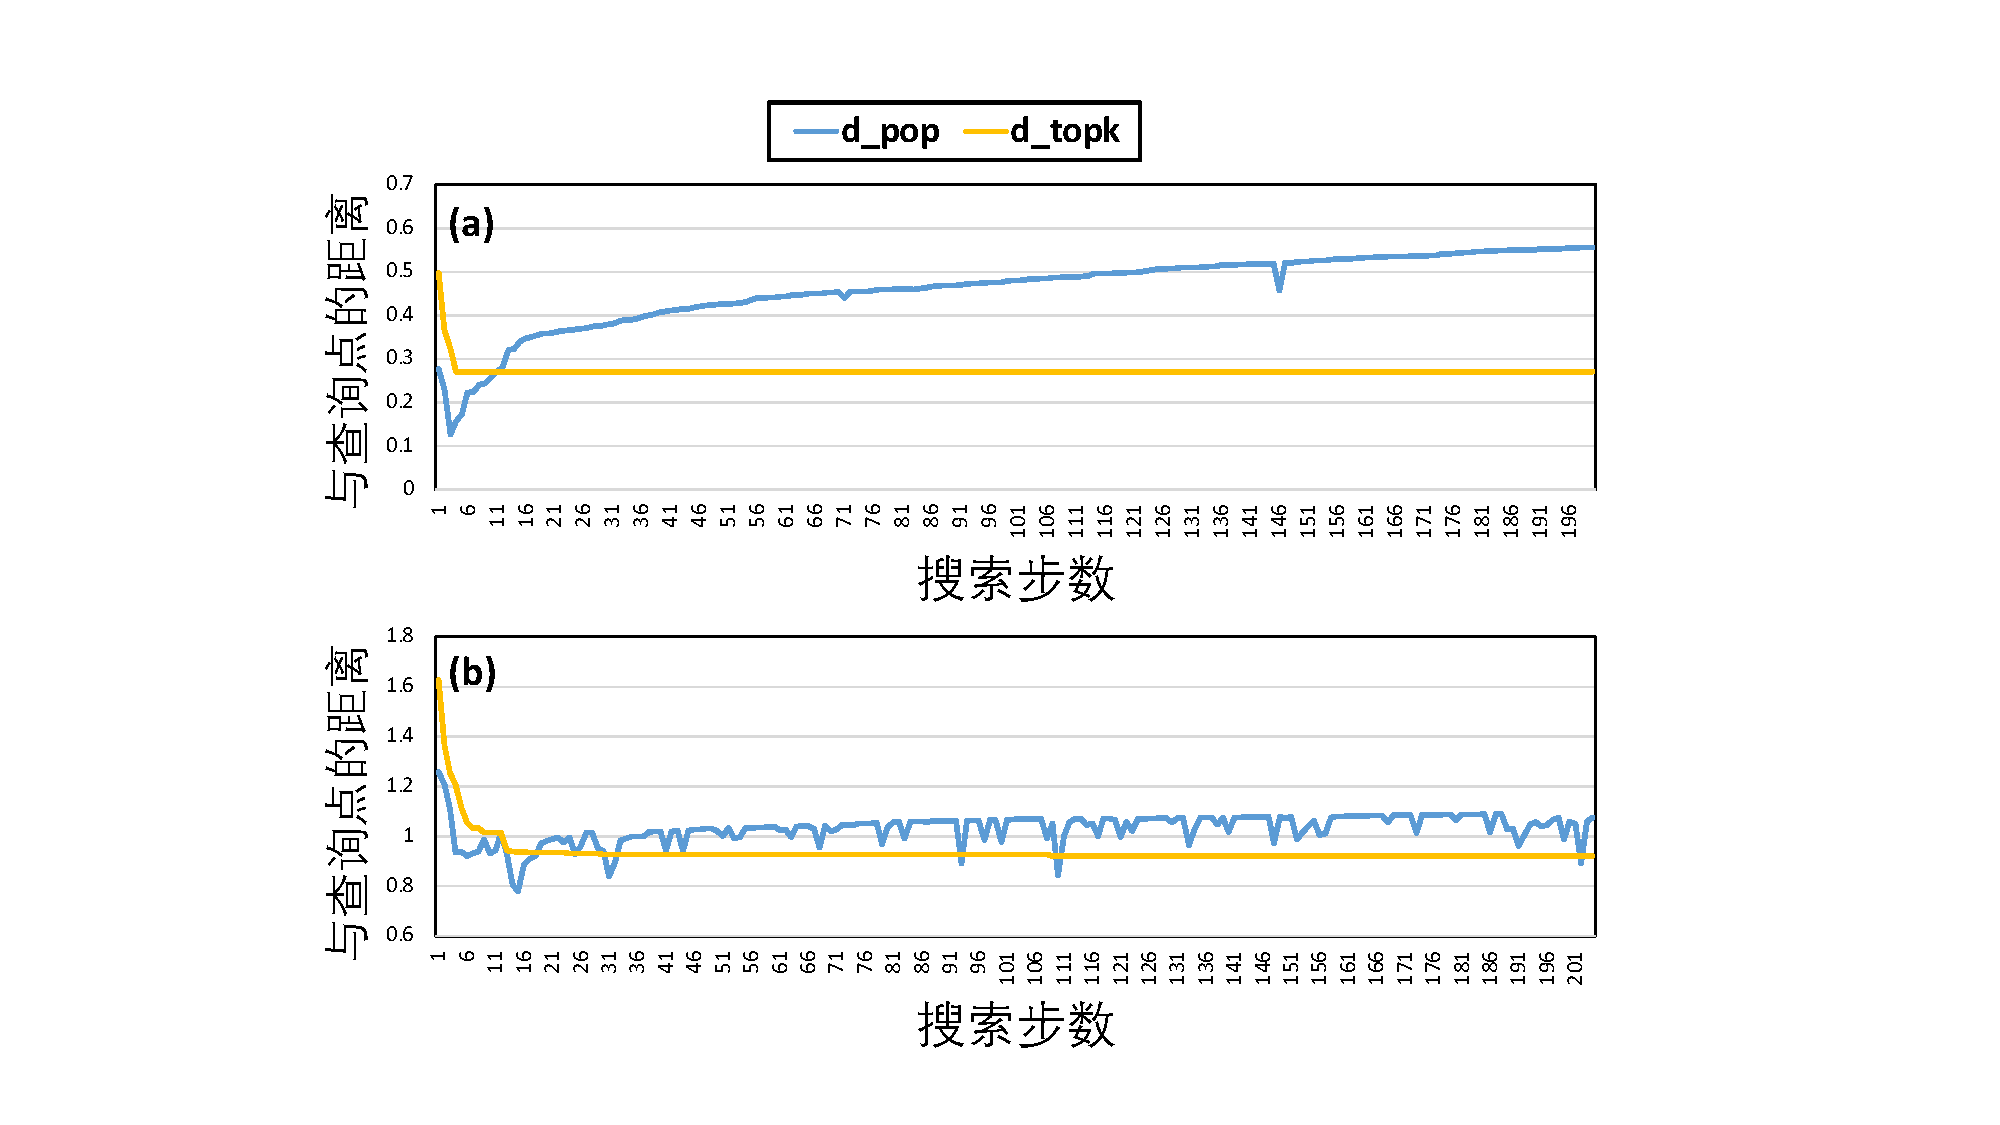
\includegraphics[width=0.6\textwidth]{figures/context-1/dist-feature.pdf}
  \caption{在搜索过程中(在DEEP1M数据集上)两个代表性查询的$d_{pop}$和$d_{topk}$的变化。(a)查询位于对称连接区域,其最小搜索步长为6。(b)查询位于非对称连接区域,其最小搜索步数为200步。}
  \label{fig:search-path}
\end{figure}

\subsection{我们的方法}
为了解决搜索过程中的冗余问题,提出了查询感知早停策略。在上述分析的基础上,我们指出$d_{pop}$相对于$d_{topk}$的曲线特征可以用来在搜索过程中识别区域。

我们通过分析$d_{pop}$相对于$d_{topk}$在搜索过程中的曲线平滑性,设计了一个预测模型来决定是否提前停止。为了消除每个查询与其最近邻居之间不一致的影响,我们另外考虑$d_{top1}$特征。我们使用的特征如下:
\begin{itemize}
    \item $d_{pop}$:当前步中,当前搜索点与查询点之间的距离。
    \item $d_{topk}$:当前步结束后,结果队列中离查询最近的点$k$ -th的距离。
    \item $d_{top1}$:当前步结束后,结果队列中最近的点到查询的距离。
\end{itemize}

对于完整的工作流(如图. \ref{fig:aware-workflow}所示),我们不需要向图索引添加任何额外的结构。在训练阶段(图~\ref{fig:aware-workflow}(a)),我们使用学习向量作为训练集(也将其划分为验证集)。对于训练集中的每个数据,我们都将按照上述搜索算法执行一个完整的搜索过程。
我们可以很容易地得到每一步的距离($d_{pop}$, $d_{topk}$和$d_{top1}$),作为预测模型的训练特征。然后我们计算最小搜索步长,并将其与曲线长度进行比较以获得标签。Label =1表示“继续搜索”,Label =0表示“终止搜索”。
在推理阶段(图~\ref{fig:aware-workflow}(b)),我们收集搜索过程中的动态特征,并通过训练好的预测模型预测剩余的搜索步数。
\begin{figure}[tp]
  \centering
  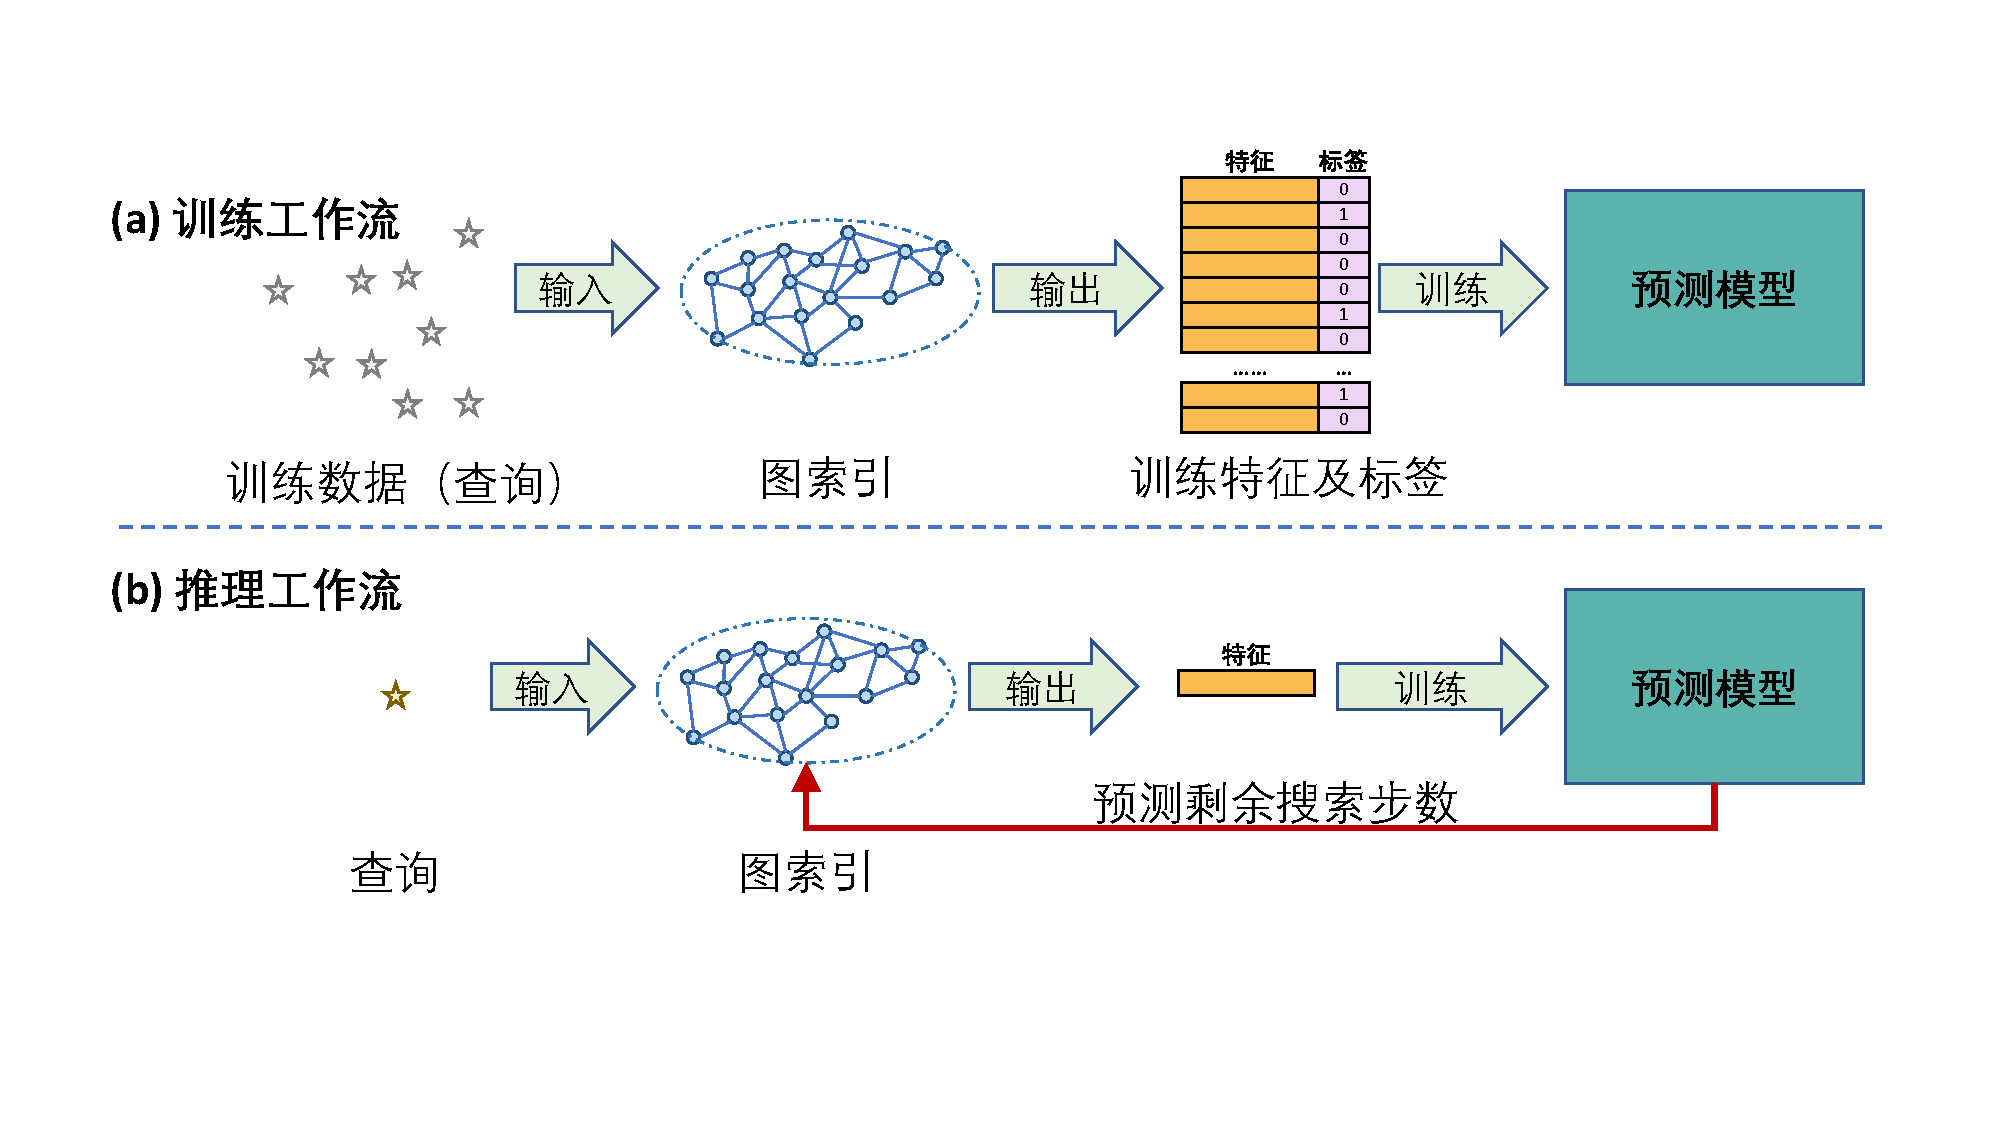
\includegraphics[width=0.7\textwidth]{figures/context-1/aware-workflow.pdf}
  \caption{支持查询感知的早停策略的工作流。(a)训练工作流,首先使用采样数据在图索引上进行搜索,然后在搜索过程中使用得到的动态特征来训练预测模型。(b)推理工作流,将训练好的模型集成到图索引框架中,在查询搜索过程中动态预测剩余搜索步数。}
  \label{fig:aware-workflow}
\end{figure}

预测模型的训练过程主要通过分析$d_{pop}$序列的平滑性来决定是否停止搜索过程。具体过程如下:(1)求$d_{pop}$曲线与$d_{topk}$曲线的上升交点步长。如果从$st_{stable}$ -th阶跃开始,$d_{pop}$大于$d_{topk}$,则$st_{stable}$称为上升交叉阶跃。(2)获取$d_{pop}$序列。从$st_{stable}$ -th步骤开始,在接下来的每一步中,$d_{pop}$添加到$d_{pop}$序列中,直到$d_{pop}$和$d_{topk}$之间的差大于$d_{topk}$和$d_{top1}$之间的差。(3)对$d_{pop}$序列进行逐差运算。对于$d_{pop}$序列,我们对其进行$n$逐差运算(类似于连续曲线的$n$阶导数)。(4) $d_{pop}$序列的方差与阈值比较。最后,我们计算$d_{pop}$序列的方差,并将其与一定阈值$th_{dist}$进行比较。如果大于阈值,则输出“继续搜索”,否则输出“终止搜索”。在实际搜索过程(推理阶段)中,我们可以轻松地收集这些距离作为预测的特征。

\begin{figure}[tp]
  \centering
  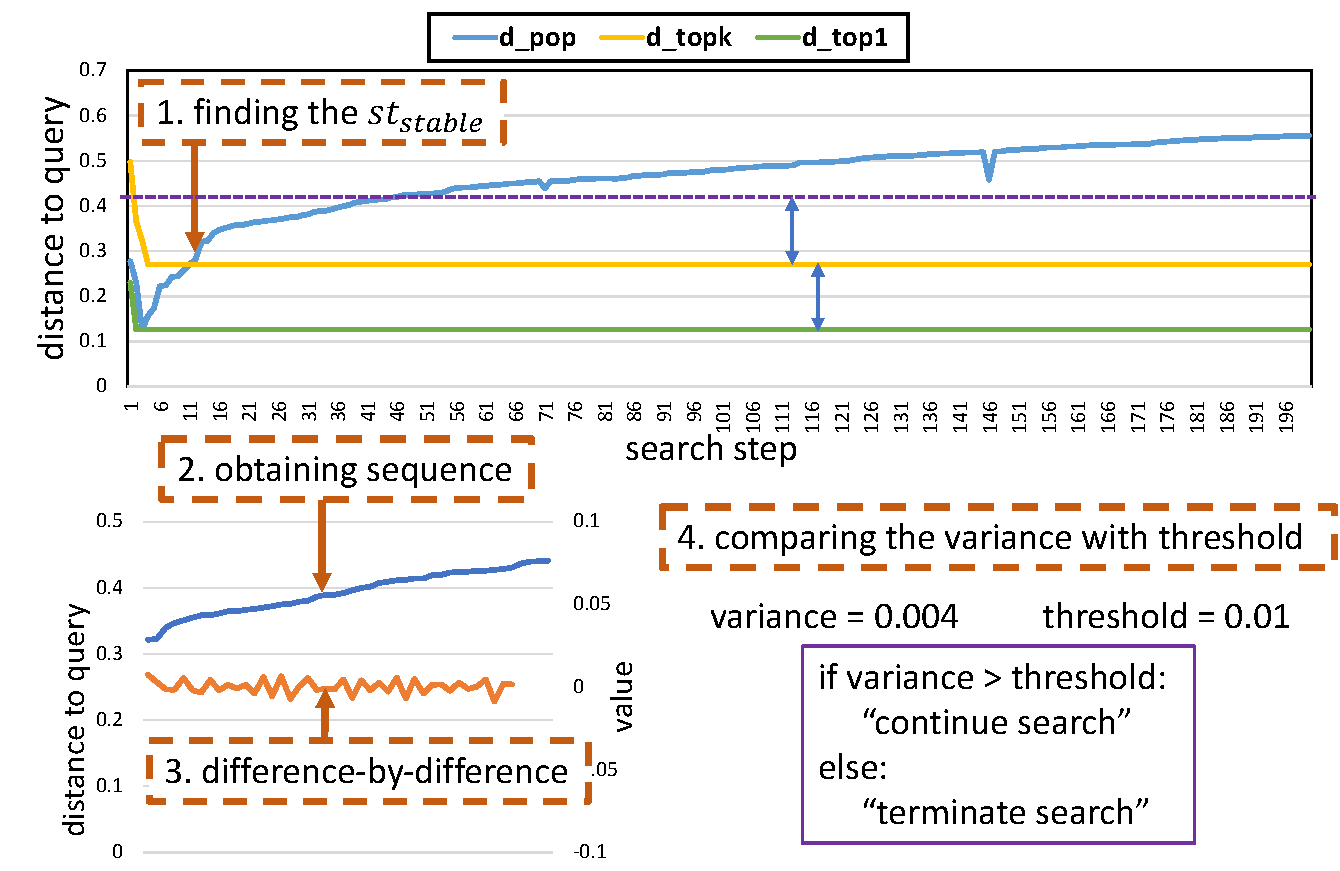
\includegraphics[width=0.7\textwidth]{figures/context-1/prediction model.pdf}
  \caption{预测模型的整个流程。它由4个步骤组成:(1)找到$st_{stable}$,(2)获得序列,(3)逐差,(4)方差与阈值比较。}
  \label{fig:prediction-model}
\end{figure}


\section{实验结果}\label{sec:galg-experiment}
在本节中,我们首先将我们的方法与最先进的近似近邻搜索方法进行比较。通过消融研究进一步分析每种技术的贡献。对于每个数据集和方法,进行多次实验,以获得稳定可靠的结果。

\subsection{实验设置和数据集}
\subsubsection{数据集}
我们使用的数据集如表~\ref{tab:datasets}所示,这些数据集在近似近邻搜索方法中被广泛使用。\ganns 方法将基础数据构建为图索引,并在该图索引上搜索查询数据的$k$最近邻。原始数据集包含10亿数据,我们截取前100万/ 1000万数据作为底库数据集。对于DEEP数据集,我们从其余数据中截取一些数据作为训练数据集(用于训练预测模型)。
\begin{itemize}
    % \item SIFT1M/10M \footnote{\label{bigann}http://corpus-texmex.irisa.fr/}: SIFT dataset consists of SIFT descriptors extracted from a large image dataset, and each data is a 128-dimensional vector.
    \item DEEP1M/10M \cite{deep-2016}:DEEP数据集来自深度分类图像模型GoogLeNet,每个数据都是一个96维向量。
    \item Turing1M/10M \cite{billionanns}:Turing数据集是由微软图灵团队为十亿规模的近似近邻搜索挑战赛发布的新数据集。它由图灵AGI v5编码的Bing查询组成,每个数据都是一个100维向量。
    % \item GIST1M \footref{bigann}: GIST dataset consists of GIST descriptors extracted from a image dataset, and each data is a 960-dimensional vector.
\end{itemize}

\begin{table}[htbp]
  \centering
  \caption{数据集信息}
  \label{tab:datasets}
  \begin{tabular}{ccccc}
  \hline
  数据集名称      & 数据维度   & 底库数据集大小   & 训练集大小 & 查询集大小 \\ \hline
  % SIFT1M/10M   & 128 & \begin{tabular}[c]{@{}c@{}}1,000,000/\\ 10,000,000\end{tabular} & -     & 10,000     \\
  DEEP1M/10M   & 96  & \begin{tabular}[c]{@{}c@{}}1,000,000/\\ 10,000,000\end{tabular} & 100,000     & 10,000     \\
  Turing1M/10M & 100 & \begin{tabular}[c]{@{}c@{}}1,000,000/\\ 10,000,000\end{tabular} & -   & 100,000    \\ \hline
  % GIST1M       & 960 & 1,000,000                                                       & -           & 1,000      \\ \hline
  \end{tabular}
\end{table}

\subsubsection{基线算法}
对于的基线方法,我们在Github上采用了他们的代码,并按照他们的建议设置相关参数。在搜索过程中,我们都使用一个线程来比较算法。在构建过程中,为了节省时间,我们使用所有线程构建所有索引。
\begin{itemize}
    \item \textbf{HNSW}\footnote{https://github.com/nmslib/hnswlib}是一种著名的基于图的算法,它基于一种称为分层NSW图的结构。
% \item \textbf{DPG}\footnote{https://github.com/DBAIWangGroup/nns\_benchmark} is based on a $k$NN graph to reselect undirected edges.
    \item \textbf{NSG}\footnote{https://github.com/ZJULearning/nsg}基于$k$ NN图,然后以导航节点为起点构建展开图。
\end{itemize}

\subsection{整体性能}
在多个数据集上对最先进的算法(HNSW和NSG)和本文所提出方法进行了实验。对于NSG,我们根据其在Github上的建议设置DEEP和Turing数据集的参数(由于它们的维度相似)。在实验中,对所有数据集设置如下参数:$L$ = 40, $R$ = 50, $C$ = 500。对于HNSW,通过网格搜索为每个数据集选择搜索性能最好的参数。在实验中,对所有数据集设置如下参数:$M$ = 20, $maxM0$ = 40, $efc$ = 300。

图~\ref{fig:exper-total}显示了我们的方法与当前最先进算法的整体性能对比结果。我们分别在四个数据集(DEEP1M, DEEP10M, Turing1M和Turing10M)上比较了R@1和R@10的搜索性能。在DEEP数据集(图~\ref{fig:exper-total}(a)和图~\ref{fig:exper-total}(b))上,我们的方法在R@1的情况下表现优于HNSW。该方法在R@10上的搜索性能几乎与NSG和HNSW相当。在图灵数据集(图~\ref{fig:exper-total}(c)和图~\ref{fig:exper-total}(d))上,该方法的搜索速度分别比HNSW和NSG快1.21倍和2.71倍。

\begin{figure*}[htbp]
  \centering
  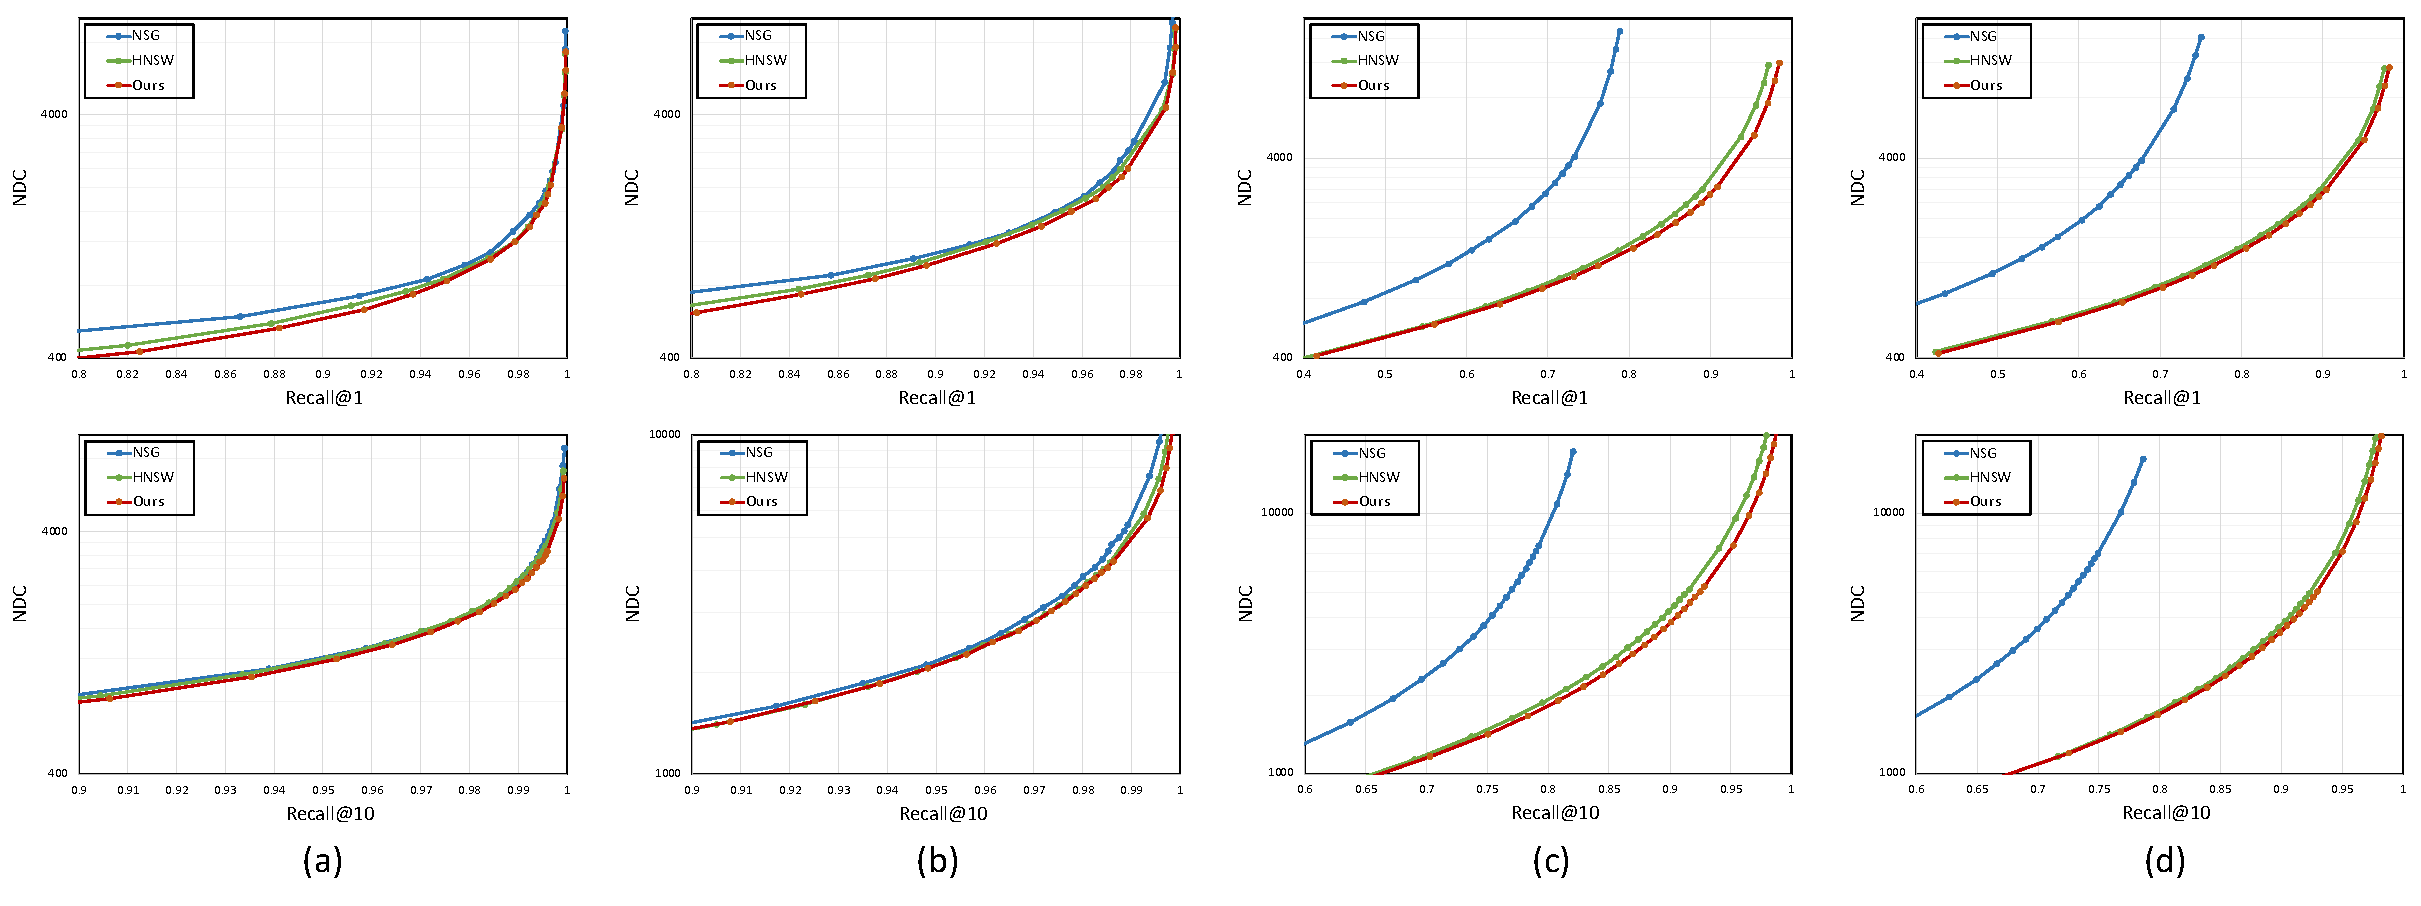
\includegraphics[width=\textwidth]{figures/context-1/exper-total.pdf}
  \caption{我们的方法分别对比HNSW和NSG算法在(a)DEEP1M,(b)DEEP10M,(c)Turing1M和(d)Turing10M 四个不同的数据集上(靠近右下更好)}
  \label{fig:exper-total}
\end{figure*}

\subsection{消融实验}
\subsubsection{反向连接增强}
在反向连接增强策略中,有两种增强模式:从候选点的随机连接部分和无法到达插入点的点。如图~\ref{fig:exper-c1}所示,我们在Turing1M数据集上将这两种策略与基线进行了比较。我们绘制了两种策略相对于基线搜索速度和基线的实际搜索速度(红色曲线)的速度。
在R@1和R@10的情况下,召回率分别为0.7、0.8和0.9。随机增强策略希望达到与基线相同的召回率,但搜索速度较慢。在R@1的情况下,我们的方法比基线分别提高了5\%,9\%和10\%的速度。这表明我们的连接增强策略在图索引上的连通性优于随机策略。
\begin{figure}[htbp]
  \centering
  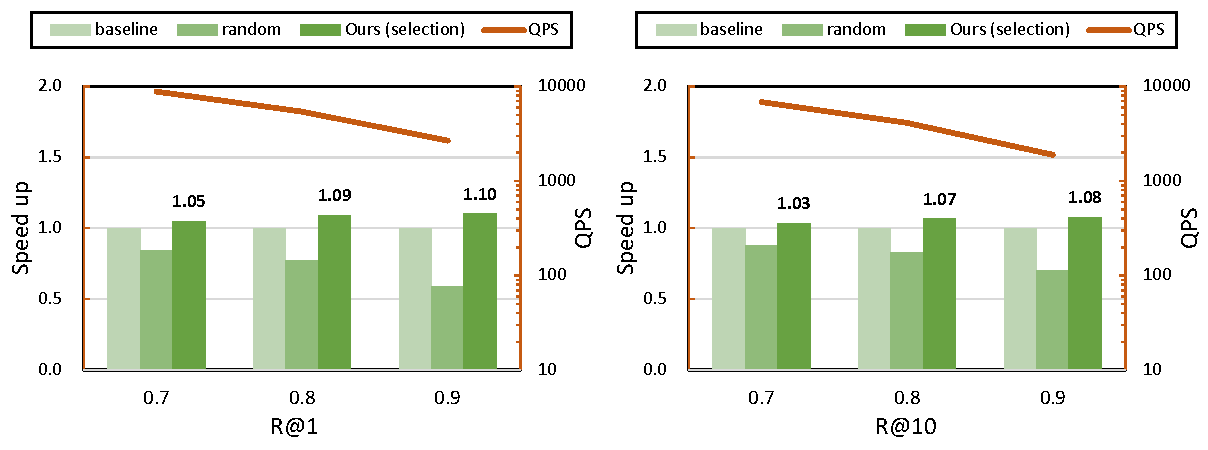
\includegraphics[width=0.7\textwidth]{figures/context-1/exper-c1.pdf}
  \caption{不同的基线反向增强和相对加速度,以及基线搜索速度。当召回率为0.9时,该策略可以加速10\%。}
  \label{fig:exper-c1}
\end{figure}


\subsubsection{查询感知策略的可扩展性}
为了证明所提出的查询感知早停策略的可扩展性,在DEEP1M和DEEP10M数据集上进行了实验。对于每个数据集,我们分别使用R@10和R@100进行实验。如表~\ref{tab:exper-c3}所示,我们分别列出了HNSW和我们的方法在DEEP数据集上实现高召回率时的NDC,以及搜索速度的比例加快。
我们发现,召回率越大,搜索速度加快的比例越大。特别地,当在DEEP1M数据集上的召回率R@10 = 0.999时,该策略可以将搜索过程加快1.29倍。在其他情况下,搜索速度有不同程度的提高。

\begin{table*}[htbp]
  \centering
  \caption{在相同召回率的情况下,采用查询感知早停策略所需的距离计算量(NDC)与基线算法的比较。}
  \label{tab:exper-c3}
  \resizebox{\textwidth}{!}{%
  \begin{tabular}{c|ccc|ccc|ccc|ccc}
  \hline
  \multirow{3}{*}{Recall rate} & \multicolumn{3}{c|}{DEEP1M-R@10} & \multicolumn{3}{c|}{DEEP1M-R@100} & \multicolumn{3}{c|}{DEEP10M-R@10} & \multicolumn{3}{c}{DEEP10M-R@100} \\ \cline{2-13} 
   & \multicolumn{2}{c}{dist.   compution} & \multirow{2}{*}{speed up} & \multicolumn{2}{c}{dist.   compution} & \multirow{2}{*}{speed up} & \multicolumn{2}{c}{dist.   compution} & \multirow{2}{*}{speed up} & \multicolumn{2}{c}{dist.   compution} & \multirow{2}{*}{speed up} \\
   & HNSW & Ours &  & HNSW & Ours &  & HNSW & Ours &  & HNSW & Ours &  \\ \hline
  0.99 & 2637.87 & 2475.86 & 1.07 & 4905.17 & 4611.04 & 1.06 & 5865.32 & 5368.36 & 1.09 & 10362.2 & 9709.18 & 1.07 \\
  0.995 & 3347.81 & 3067.41 & 1.09 & 6553.21 & 5965.97 & 1.10 & 7429.83 & 6659.18 & 1.12 & 14424.3 & 13233.8 & 1.09 \\
  0.999 & 7110.67 & 5500.62 & \textbf{1.29} & 12125.8 & 10328.2 & 1.17 & 15712.9 & 13204.6 & 1.19 & 27463.4 & 24713.9 & 1.11 \\ \hline
  \end{tabular}%
  }
\end{table*}


\section{本章小结}
本章节对\ganns 方法从近邻图角度进行了研究,指出现有方法面临的两个挑战:图连通性差和搜索存在冗余。图连通性差是由于构建算法中存在点的入度约束导致的。搜索存在冗余是由于搜索算法没有感知到查询的最小搜索步数。因此,本文提出反向连接增强策略,通过判断插入点是否可达来增加一些连接,使插入点的入度不再受限制。其次,本文提出了查询感知早停策略,通过在搜索过程中收集动态距离特征并为每个查询分配不同的搜索步数来减少搜索冗余开销。最后,通过大量实验表明,该方法可以将搜索速度提高1.06到1.29倍。